\section{Op-Amps}

\begin{frame}{Op-Amps}
    Important facts: \textbf{always applicable} (in 16A): \\[10pt]
    \begin{tabular}{m{0.5\textwidth} m{0.4\textwidth}}
        $V_{out} = G(V_+ - V_-)$ & 
        \multirow{3}{*}{
            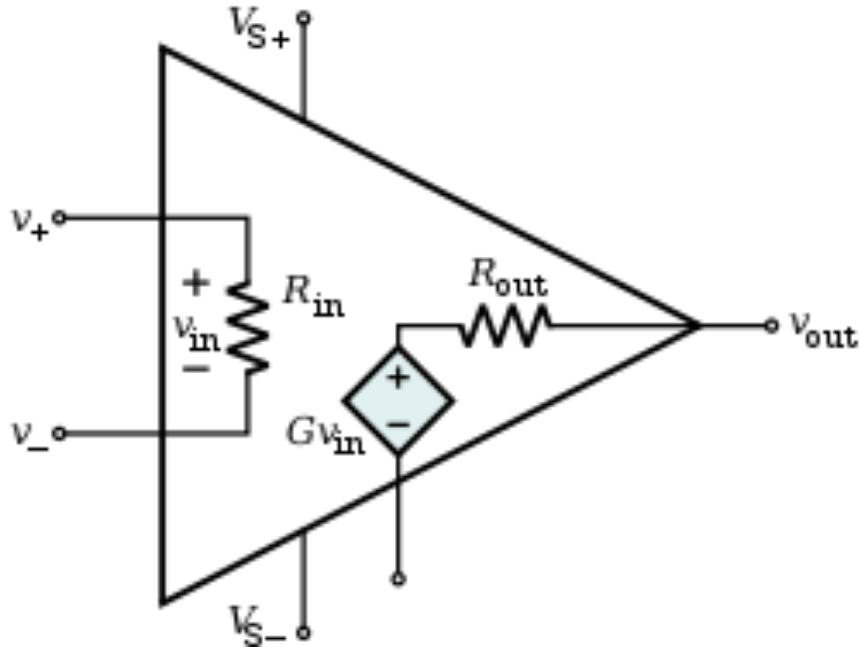
\includegraphics[width=0.45\textwidth]{images/opamp_model.png}
        } \\[5pt]
        $V_{S+} \geq V_{out} \geq V_{S-}$ & \\[10pt]
        The last fact says that the output voltage \textbf{“clips” if the input voltage difference is too large}.
    \end{tabular}
\end{frame}

\begin{frame}{Op-Amps: Gain}
    \begin{tabular}{m{0.5\textwidth} m{0.4\textwidth}}
        \textbf{Gain} can be defined differently depending on the problem. & 
        \multirow{3}{*}{
            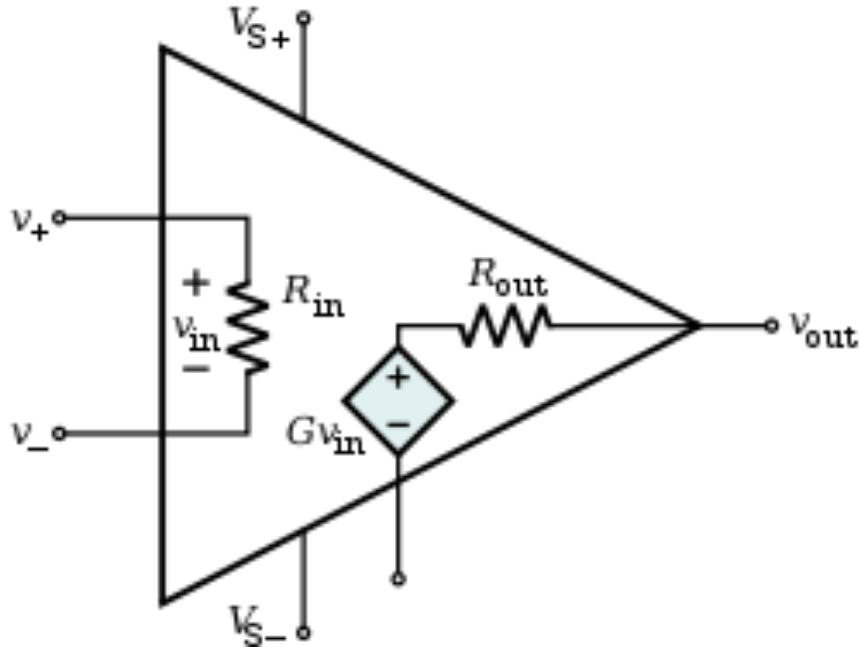
\includegraphics[width=0.45\textwidth]{images/opamp_model.png}
        } \\[20pt]
        Sometimes gain is just defined as the \textbf{ratio} of $V_{out}$ to $V_+ - V_-$. & \\[20pt]
        Other times, with a \textit{single voltage source} $V_{in}$, it can be defined as the ratio of $V_{out}$ to $V_{in}$. & \\[25pt]
    \end{tabular}
    Usually, “gain” refers to \textbf{voltage gain}, and will be $G = V_{out}/V_{in}$.
\end{frame}

\begin{frame}{Comparators}
    A device that \textbf{compares two voltages} and outputs a digital signal indicating which is larger. \\
    \begin{tabular}{m{0.5\textwidth} m{0.4\textwidth}}
        An \textbf{op-amp} can act as a comparator because, when $V_+ > V_-$, it outputs $V_{S+}$, and when $V_+ < V_-$, it output $V_{S-}$. & 
        \begin{circuitikz}[scale=0.8, transform shape]
            \draw (0, 0) node[op amp] (opamp) {}
            (opamp.-) to[short, -o] (-1.5, 0.5) node[label={left:$-$ input}] {}
            (opamp.+) to[short, -o] (-1.5, -0.5) node[label={left:$+$ input}] {}
            (opamp.out) to[short, -o] (1.5, 0) node[label={right: output}] {}
            (opamp.up) to[short] (-0.1, 1.5) node[vdd, label={left: $V_{S+}$}] {}
            (opamp.down) to[short] (-0.1, -1.5) node[vss, label={left: $V_{S-}$}] {};
        \end{circuitikz}
    \end{tabular}
\end{frame}

\begin{frame}{Golden Rules}
    \begin{tabular}{m{0.5\textwidth} m{0.4\textwidth}}
        & 
        \multirow{5}{*}{
            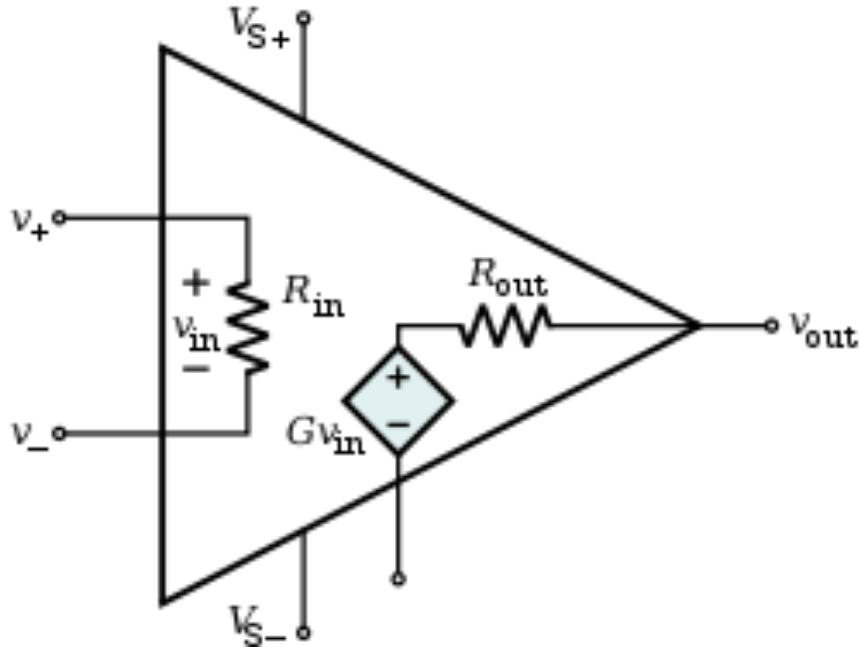
\includegraphics[width=0.45\textwidth]{images/opamp_model.png}
        } \\
        For \textbf{ideal op-amps}, take & \\
        $G \to \infty,\, R_{in} \to \infty,\, R_{out} \to 0$ & \\[10pt]
        For all ideal op-amps, \textbf{input terminals draw no current}: & \\[5pt]
        $I_- = I_+ = 0$ & \\[25pt]
    \end{tabular}
    For all ideal op-amps in \textbf{negative feedback}, there is \textbf{no voltage difference} between the two input teminals: $V_- = V_+$
\end{frame}